% This is samplepaper.tex, a sample chapter demonstrating the
% LLNCS macro package for Springer Computer Science proceedings;
% Version 2.20 of 2017/10/04
%
\documentclass[runningheads]{llncs}
%
\usepackage{graphicx}
% Used for displaying a sample figure. If possible, figure files should
% be included in EPS format.
%
% If you use the hyperref package, please uncomment the following line
% to display URLs in blue roman font according to Springer's eBook style:
% \renewcommand\UrlFont{\color{blue}\rmfamily}

\begin{document}
%
\title{Marlowe: implmenting and analysing financial contracts\thanks{Supported by IOHK.}}
%
%\titlerunning{Abbreviated paper title}
% If the paper title is too long for the running head, you can set
% an abbreviated paper title here
%
\author{
Pablo Lamela Seijas\inst{1} \and
Alex Nemish\inst{1} \and
David Smith\inst{1} \and
Simon Thompson\inst{1,2}\orcidID{0000-0002-2350-301X}}
%
\authorrunning{P. L. Seijas, A. Nemish, et al.}

% First names are abbreviated in the running head.
% If there are more than two authors, 'et al.' is used.
%
\institute{IOHK, Hong Kong, \url{https://iohk.io} \\
\email{\{alexander.nemish, pablo.lamela, david.smith, simon.thompson\}@iohk.io} \and
School of Computing, University of Kent, UK\\
\email{s.j.thompson@kent.ac.uk}}
%
\maketitle              % typeset the header of the contribution
%



\begin{abstract}
The abstract should briefly summarize the contents of the paper in
150--250 words.

\keywords{First keyword  \and Second keyword \and Another keyword.}
\end{abstract}
%
%
%


\section{Introduction}

Intro
\section{Marlowe overview SJT}

Introduce the main types and informal overview of execution. Contrast with Marlowe 1.3 (as in ISoLA paper). Embedding in Haskell? [All this stuff is in the tutorial already]

\section{Implementation of Marlowe on the mockchain AN}

 [An updated version of the description in the Plutus platform paper]

\section{Analysing Marlowe contracts PLS}

Covers static analysis and Isabelle proofs [New]


\section{The Marlowe Playground DS}

[There's some stuff on this in the tutorial.]

\section{Related work}

Need to update from ISoLA paper \cite{isola-marlowe}.

\section{Future work and conclusions}

\section*{Left in for info \ldots}

%\begin{figure}
%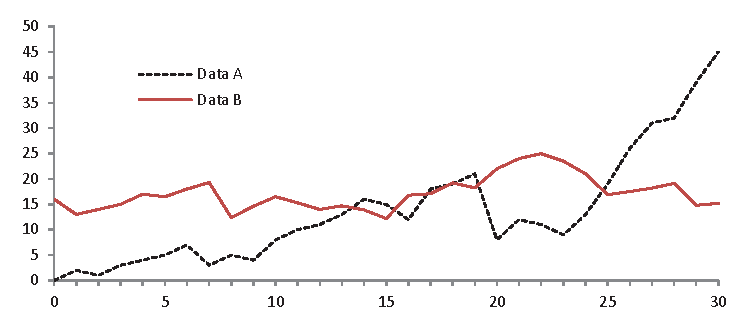
\includegraphics[width=\textwidth]{fig1.eps}
%\caption{A figure caption is always placed below the illustration.
%Please note that short captions are centered, while long ones are
%justified by the macro package automatically.} \label{fig1}
%\end{figure}


%
% ---- Bibliography ----
%
% BibTeX users should specify bibliography style 'splncs04'.
% References will then be sorted and formatted in the correct style.
%
\bibliographystyle{splncs04}
\bibliography{paper}
%
\end{document}
